\documentclass[journal]{IEEEtran}

% *** CITATION PACKAGES ***
%
%\usepackage{cite}
\usepackage{capt-of}%%To get the caption
\usepackage{gensymb}
\usepackage{graphicx} %package to manage images
\graphicspath{ {./images/} }
\usepackage{wrapfig}

\usepackage[style=ieee]{biblatex}
\DeclareLanguageMapping{english}{english-apa}
\addbibresource{references.bib}
\usepackage[justification=centering]{caption}

\usepackage{setspace}

\usepackage{hhline}

\usepackage{booktabs}
\usepackage{xcolor}

\usepackage{makecell}

\renewcommand\theadfont{}

\raggedbottom

% *** GRAPHICS RELATED PACKAGES ***
%
\ifCLASSINFOpdf
  % \usepackage[pdftex]{graphicx}
  % declare the path(s) where your graphic files are
  % \graphicspath{{../pdf/}{../jpeg/}}
  % and their extensions so you won't have to specify these with
  % every instance of \includegraphics
  % \DeclareGraphicsExtensions{.pdf,.jpeg,.png}
\else
  % or other class option (dvipsone, dvipdf, if not using dvips). graphicx
  % will default to the driver specified in the system graphics.cfg if no
  % driver is specified.
  % \usepackage[dvips]{graphicx}
  % declare the path(s) where your graphic files are
  % \graphicspath{{../eps/}}
  % and their extensions so you won't have to specify these with
  % every instance of \includegraphics
  % \DeclareGraphicsExtensions{.eps}
\fi
% graphicx was written by David Carlisle and Sebastian Rahtz. It is
% required if you want graphics, photos, etc. graphicx.sty is already
% installed on most LaTeX systems. The latest version and documentation
% can be obtained at: 
% http://www.ctan.org/pkg/graphicx
% Another good source of documentation is "Using Imported Graphics in
% LaTeX2e" by Keith Reckdahl which can be found at:
% http://www.ctan.org/pkg/epslatex
%
% latex, and pdflatex in dvi mode, support graphics in encapsulated
% postscript (.eps) format. pdflatex in pdf mode supports graphics
% in .pdf, .jpeg, .png and .mps (metapost) formats. Users should ensure
% that all non-photo figures use a vector format (.eps, .pdf, .mps) and
% not a bitmapped formats (.jpeg, .png). The IEEE frowns on bitmapped formats
% which can result in "jaggedy"/blurry rendering of lines and letters as
% well as large increases in file sizes.
%
% You can find documentation about the pdfTeX application at:
% http://www.tug.org/applications/pdftex

\begin{document}

\begin{titlepage}
    {\centering
        \vspace*{20em}
        {
        \huge 
        \begin{spacing}{1.5}
            Lab Report \#2: RLC Circuits
            \\
            Advanced Circuits Lab (ENGR$-$UH 2311),\\
            Spring 2019
            \bigskip
            \Large
            \\
            Determining the Characteristics of Simple Resistor,\\
            Inductor, and Capacitor Circuits
  
            \\
            \bigskip
            Deadline: April 24, 2019 
        \end{spacing}

        }
        
    }
    \vfill
    
    {
    \large
    
    \begin{spacing}{1.5}
    \noindent Barkin Simsek, {\it {bs3528@nyu.edu}} 
    \\
    Nishant Aswani, {\it {nsa325@nyu.edu}}
    \\
    Section \#1% <-this % stops a space
    \\
    Workstation \#8% <-this % stops a space
    \end{spacing}
    }


\end{titlepage}
\pagenumbering{gobble}
%\clearpage\mbox{} % adds and empty page
%\clearpage
\pagenumbering{arabic}
\setcounter{page}{1}

%\title{Demonstration of a Voltage Divider With A Variable Resistor}

%\author{Barkin Simsek,~\IEEEmembership{bs3528@nyu.edu};
%Nishant Aswani,~\IEEEmembership{nsa325@nyu.edu}
%\\ Table Number: \#}% <-this % stops a space


% The paper headers
\markboth{Simsek, Aswani, Advanced Circuits Lab 2019}%
{}

% make the title area
%\maketitle

% As a general rule, do not put math, special symbols or citations
% in the abstract or keywords.
\begin{abstract}
Lorem ipsum dolor sit amet, consectetur adipiscing elit. Nullam ultrices feugiat risus eget tincidunt. Integer nibh erat, luctus sed consectetur eu, dapibus ac nisi. Sed convallis mi eu risus ullamcorper dictum. Proin iaculis velit at massa pellentesque, sed congue dolor aliquam. Aenean rutrum vel mauris a malesuada. Nam posuere sagittis.\\

Lorem ipsum dolor sit amet, consectetur adipiscing elit. Nullam ultrices feugiat risus eget tincidunt. Integer nibh erat, luctus sed consectetur eu, dapibus ac nisi. Sed convallis mi eu risus ullamcorper dictum. Proin iaculis velit at massa pellentesque, sed congue dolor aliquam. Aenean rutrum vel mauris a malesuada. Nam posuere sagittis.\\
\end{abstract}

%Percenta of power being consumed at the internal resistence

%What happens to voltage when external load is connected and current %consumption increaased

%Formula derivation
%Application 


\section{Introduction}

\IEEEPARstart{T}\lowercase{he} goal of this lab was to prototype inductor and capacitor circuits and gain an understanding of leading/lagging, the effect of frequency on phase shifts, and the idea of resonance frequency. \\


\noindent Inductors and capacitors are both energy storage elements capable of phase-shifting input signals. An inductor operates on the principal of storing energy as a magnetic field and opposes rapid changes in current, acting as a filter for high frequency signals. Capacitors collect charge on their plates, storing energy in the form of electric fields between their plates; they act as a filter for low frequency signals. \\

\noindent An inductor opposes high frequency signals and produces an output voltage that leads the input voltage by a phase angle of $\phi$. On the other hand, a capacitor does not oppose high frequency signals and produces an output voltage that lags the input voltage by a phase angle of $\theta$. \\

\noindent In order to demonstrate the concept of leading/lagging, three circuits were built using resistors, capacitors, and inductors. The table below summarizes the instruments used to build the circuits in this experiment. \\

\begingroup
    \medskip
\centering
\def\arraystretch{1.5}
\begin{tabular}{lc}
\toprule
Item & Quantity \\
\midrule
1K$\ohm$ Resistor & 1 \\
3.3$uF$ Capacitor & 1 \\
4.7$mH$ Inductor & 1 \\
Oscilloscope & 1 \\
Dual Output Power Supply & 1 \\
AC Function Generator & 1 \\
Solid-Core Wires & Various Lengths \\
Wire Stripper & 1 \\
\bottomrule
\end{tabular}
\captionof{figure}{Tabulation of the equipment and materials used for this experiment}
\label{fig:table}
    \medskip
\endgroup



\section{Experimental Set-up}

%%%%%%%%%%%%%%%%
%% RC Circuit %%
%%%%%%%%%%%%%%%%
\subsection{RC Circuit}
\noindent In a RC circuit, capacitor {\color{red}does something something something theory theory Lorem ipsum dolor sit amet, consectetur adipiscing elit. Nullam ultrices feugiat risus eget tincidunt. Integer nibh erat, luctus sed consectetur eu, dapibus ac nisi. Lorem ipsum dolor sit amet, consectetur adipiscing elit. Nullam ultrices feugiat risus eget tincidunt. Integer nibh erat, luctus sed consectetur eu, dapibus ac nisi.Lorem ipsum dolor sit amet, consectetur adipiscing elit. Nullam ultrices feugiat risus eget tincidunt. Integer nibh erat, luctus sed consectetur eu, dapibus ac nisi.}

\begingroup
    \centering
    \medskip
    %width=\columnwidth
    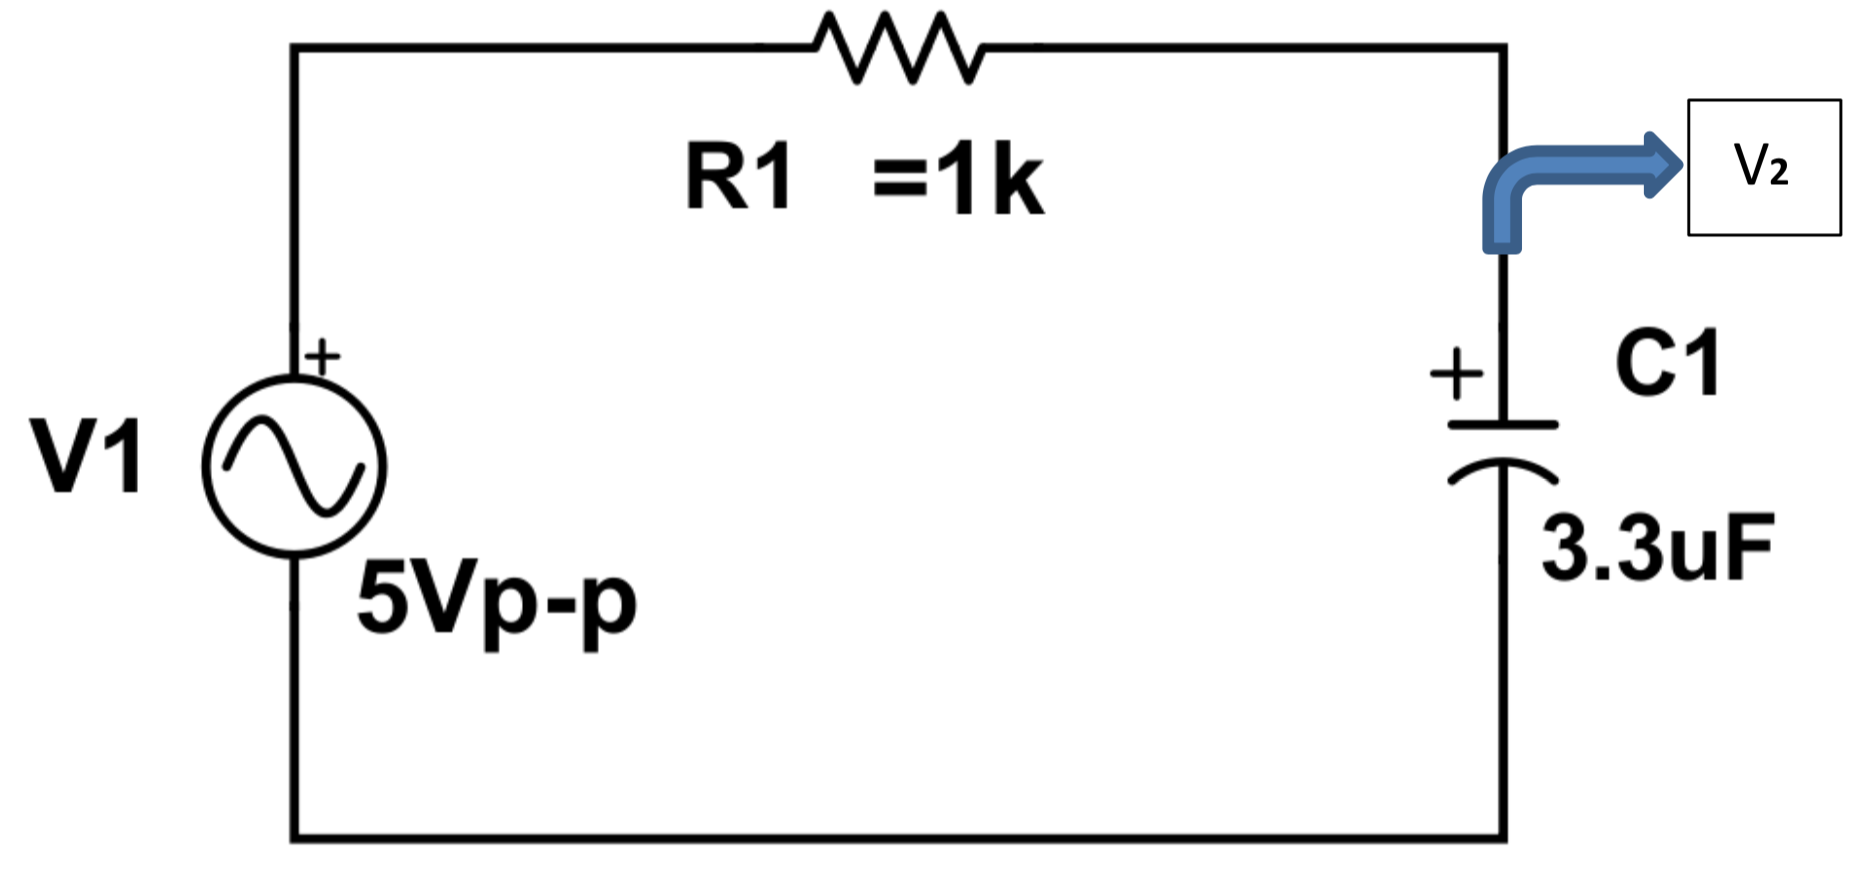
\includegraphics[width=\columnwidth]{images/lab8_circuit1.png}
    \captionof{figure}{Circuit 1}
    \label{fig:circ1}
    \medskip
\endgroup

\noindent Following the schematics above (Figure \ref{fig:circ1}), the circuit was built on a breadboard. 5V p-p AC voltage was applied to the circuit and crocodile grabbers of the oscilloscope were attached to the leg of the capacitor and the common ground of the circuit. $R1$ was selected to be \ohm and the capacitor was selected to be 3.3$uF$. Once the circuit was built as shown in Figure \ref{fig:circ1image}, 5V p-p sinusoidal wave at 1 kHz and 2 kHz was applied. The phase shift difference between the originally supplied sinusoidal wave and the waveform at the leg of the capacitor was measured using the cursor functionality of the oscilloscope. Later, the frequency of the waveform was increased up to 40 kHz to observe the change in the phase shift.

\begingroup
    \centering
    \medskip
    %width=\columnwidth
    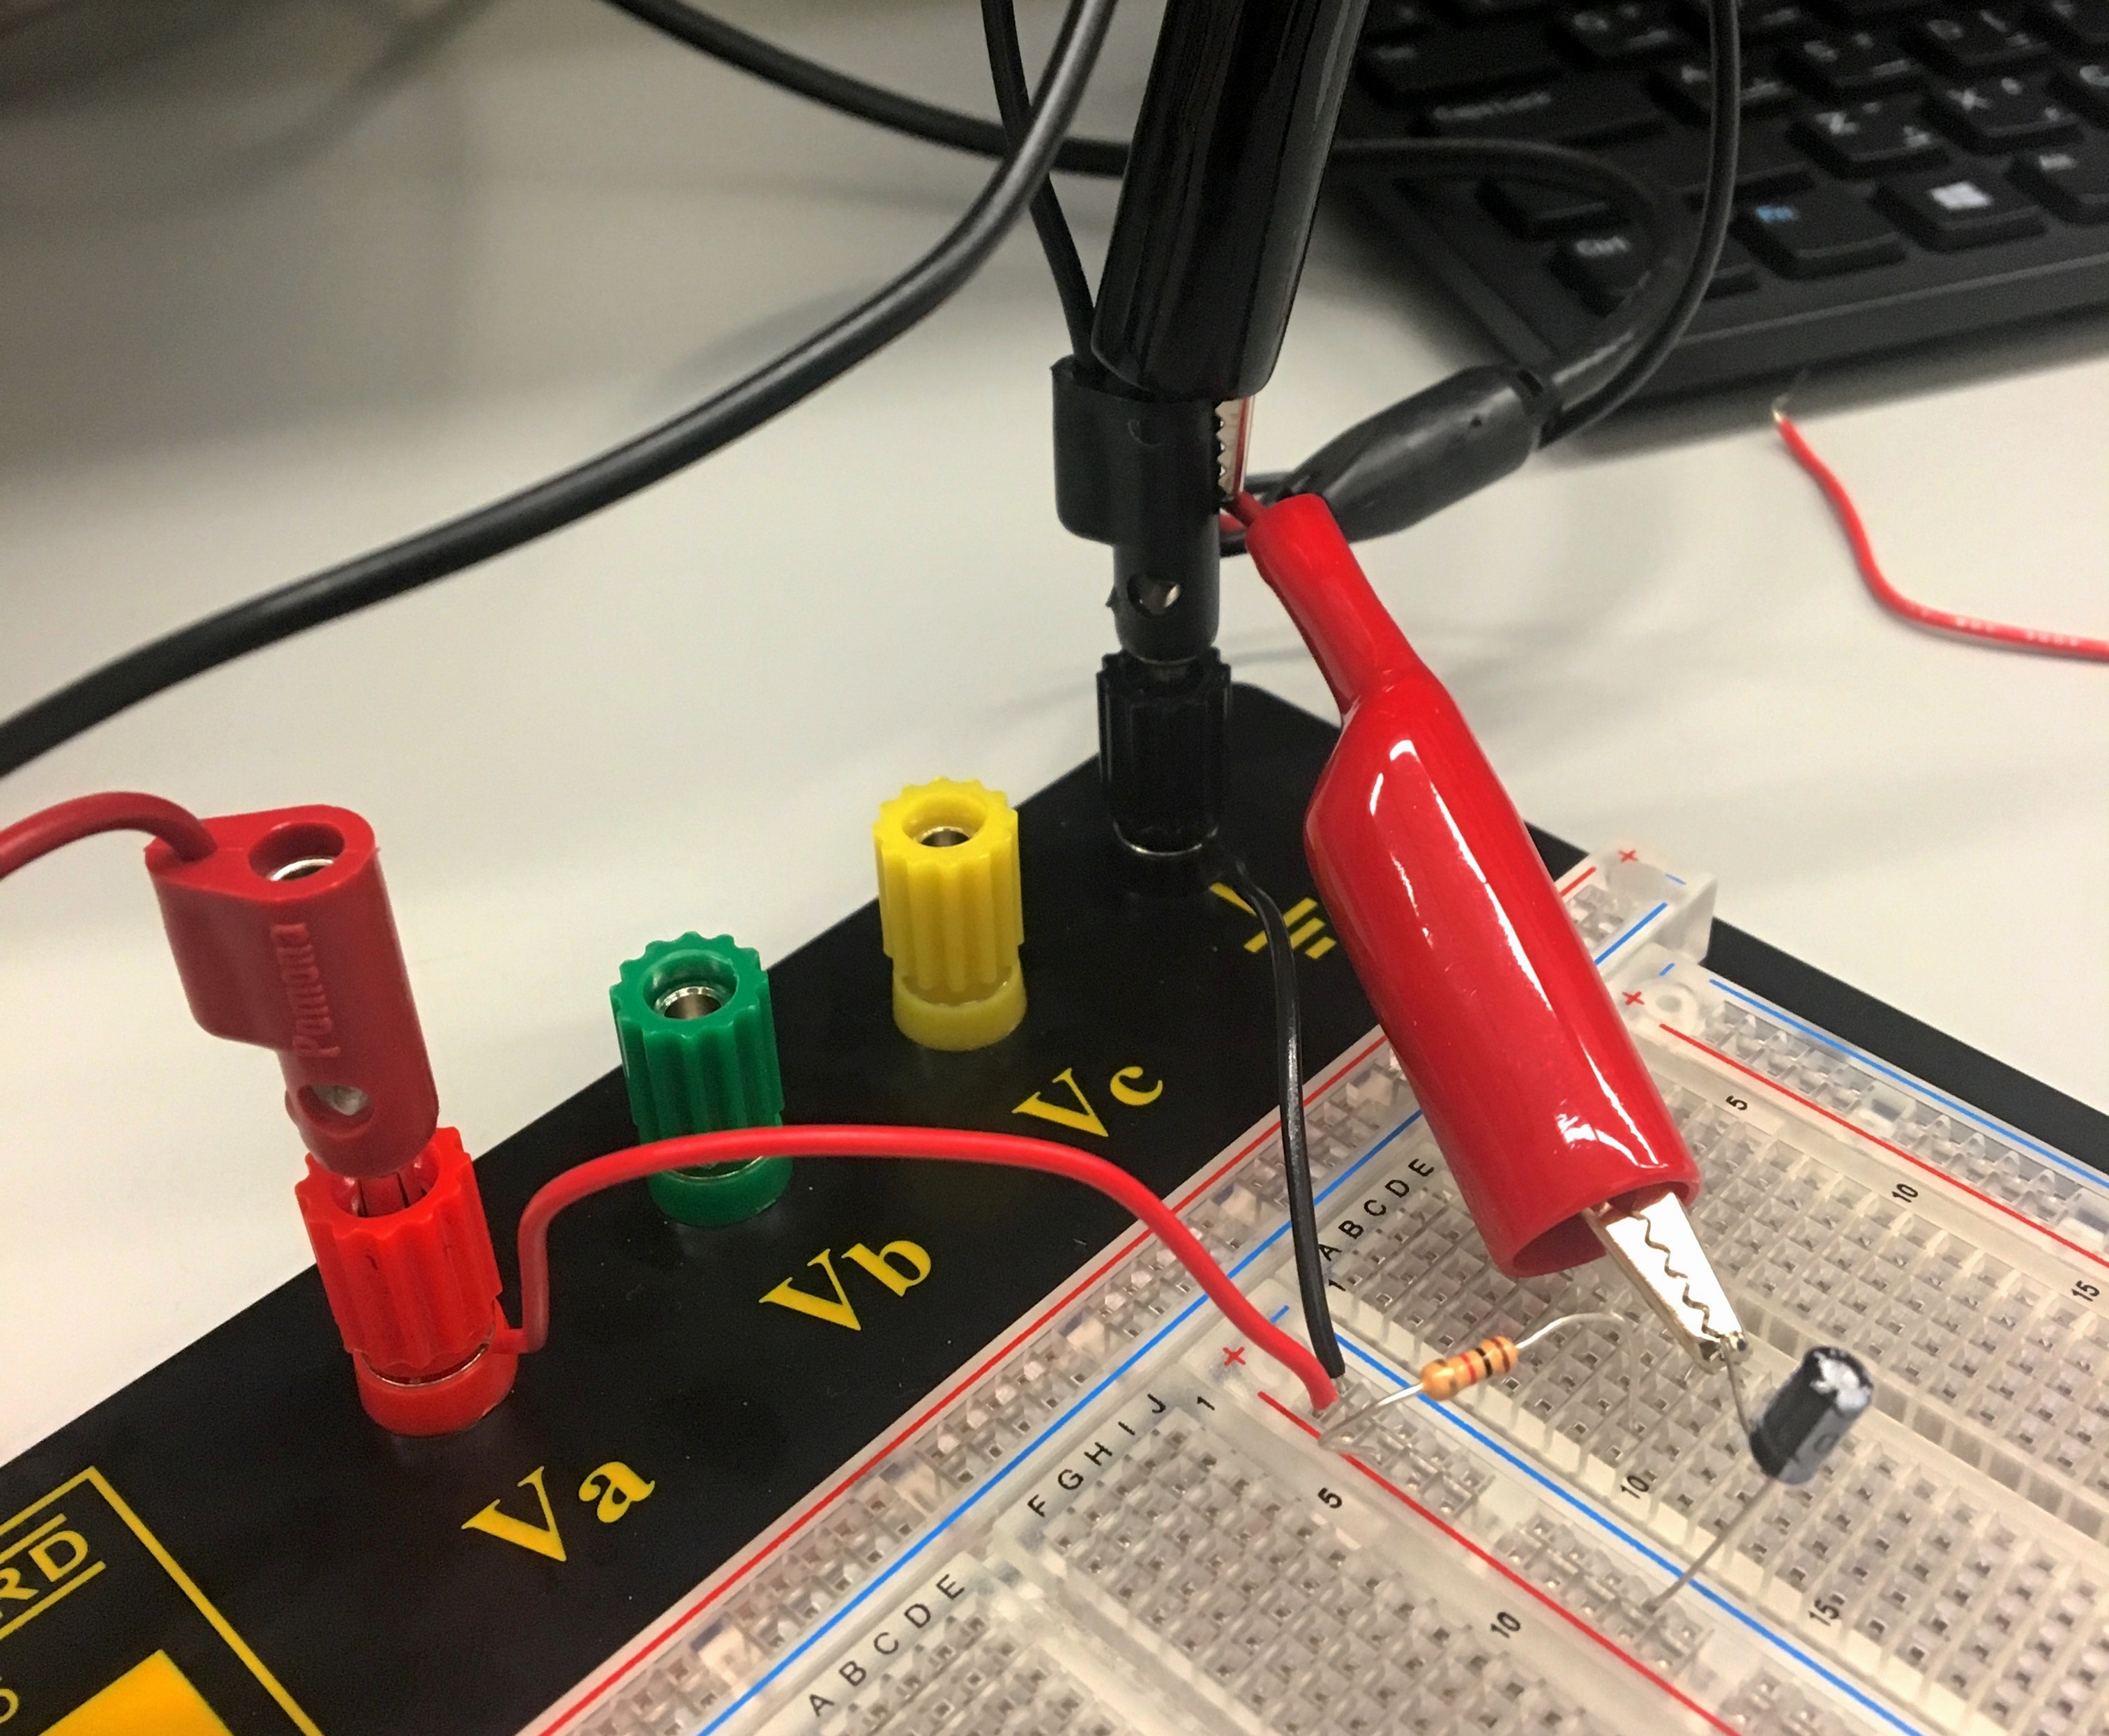
\includegraphics[width=\columnwidth]{images/lab8_circ1.jpg}
    \captionof{figure}{Circuit 1}
    \label{fig:circ1image}
    \medskip
\endgroup



%%%%%%%%%%%%%%%%
%% RL Circuit %%
%%%%%%%%%%%%%%%%
\subsection{RL Circuit}
\noindent In a RL circuit, inductor {\color{red}does something something something theory theory Lorem ipsum dolor sit amet, consectetur adipiscing elit. Nullam ultrices feugiat risus eget tincidunt. Integer nibh erat, luctus sed consectetur eu, dapibus ac nisi.Lorem ipsum dolor sit amet, consectetur adipiscing elit. Nullam ultrices feugiat risus eget tincidunt. Integer nibh erat, luctus sed consectetur eu, dapibus ac nisi.} 

\begingroup
    \centering
    \medskip
    %width=\columnwidth
    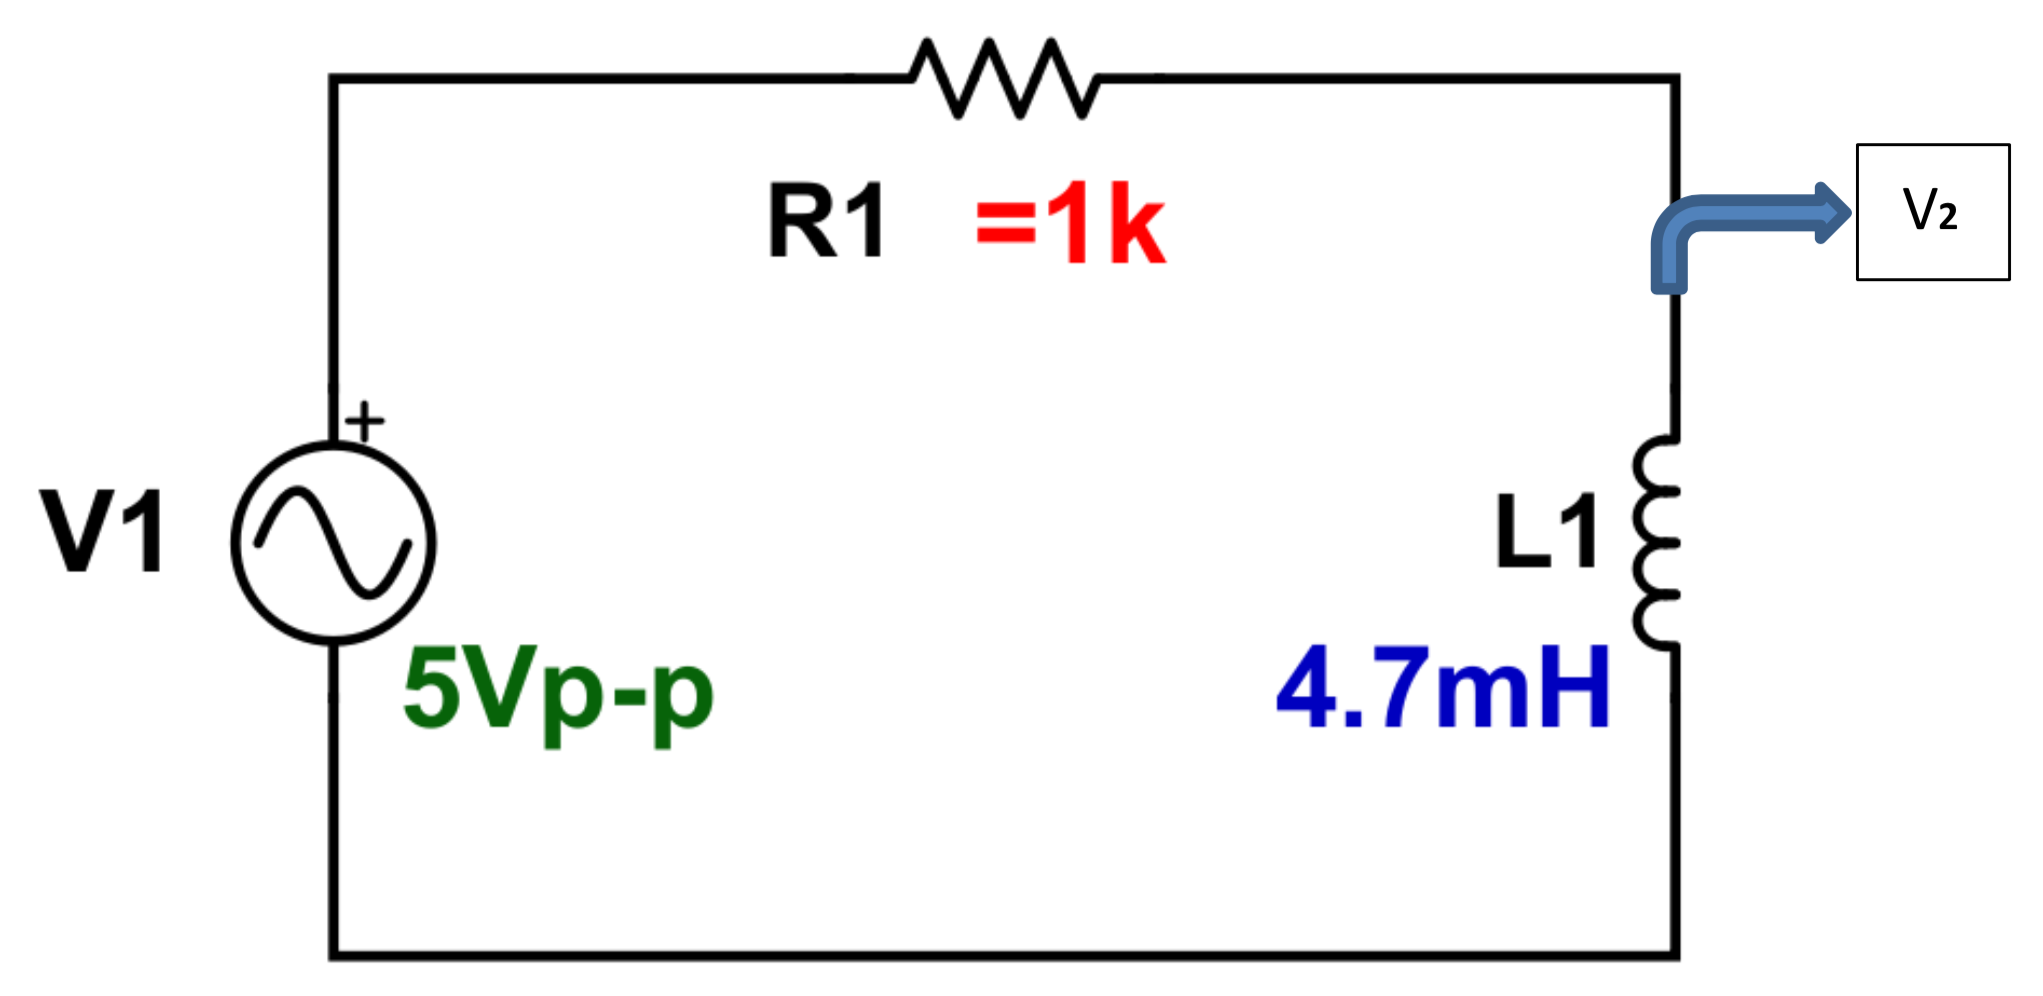
\includegraphics[width=\columnwidth]{images/lab8_circuit2.png}
    \captionof{figure}{Circuit 2}
    \label{fig:circ2}
    \medskip
\endgroup

\noindent Following the schematics provided (Figure \ref{fig:circ2}), the circuit was built on a breadboard. 5V p-p AC voltage was applied to the circuit and crocodile grabbers of the oscilloscope were attached to the leg of the inductor and the common ground of the circuit. One 4.7 $mH$ inductor and one 1K \ohm resistor was used in the circuit. After the circuit was completed as shown in Figure \ref{fig:circ2image}, the magnitude of the voltage and phase difference between the supplied wave and the waveform captured from the leg of the inductor. The measurements were repeated for 1kHz and 2 kHz frequencies.

\begingroup
    \centering
    \medskip
    %width=\columnwidth
    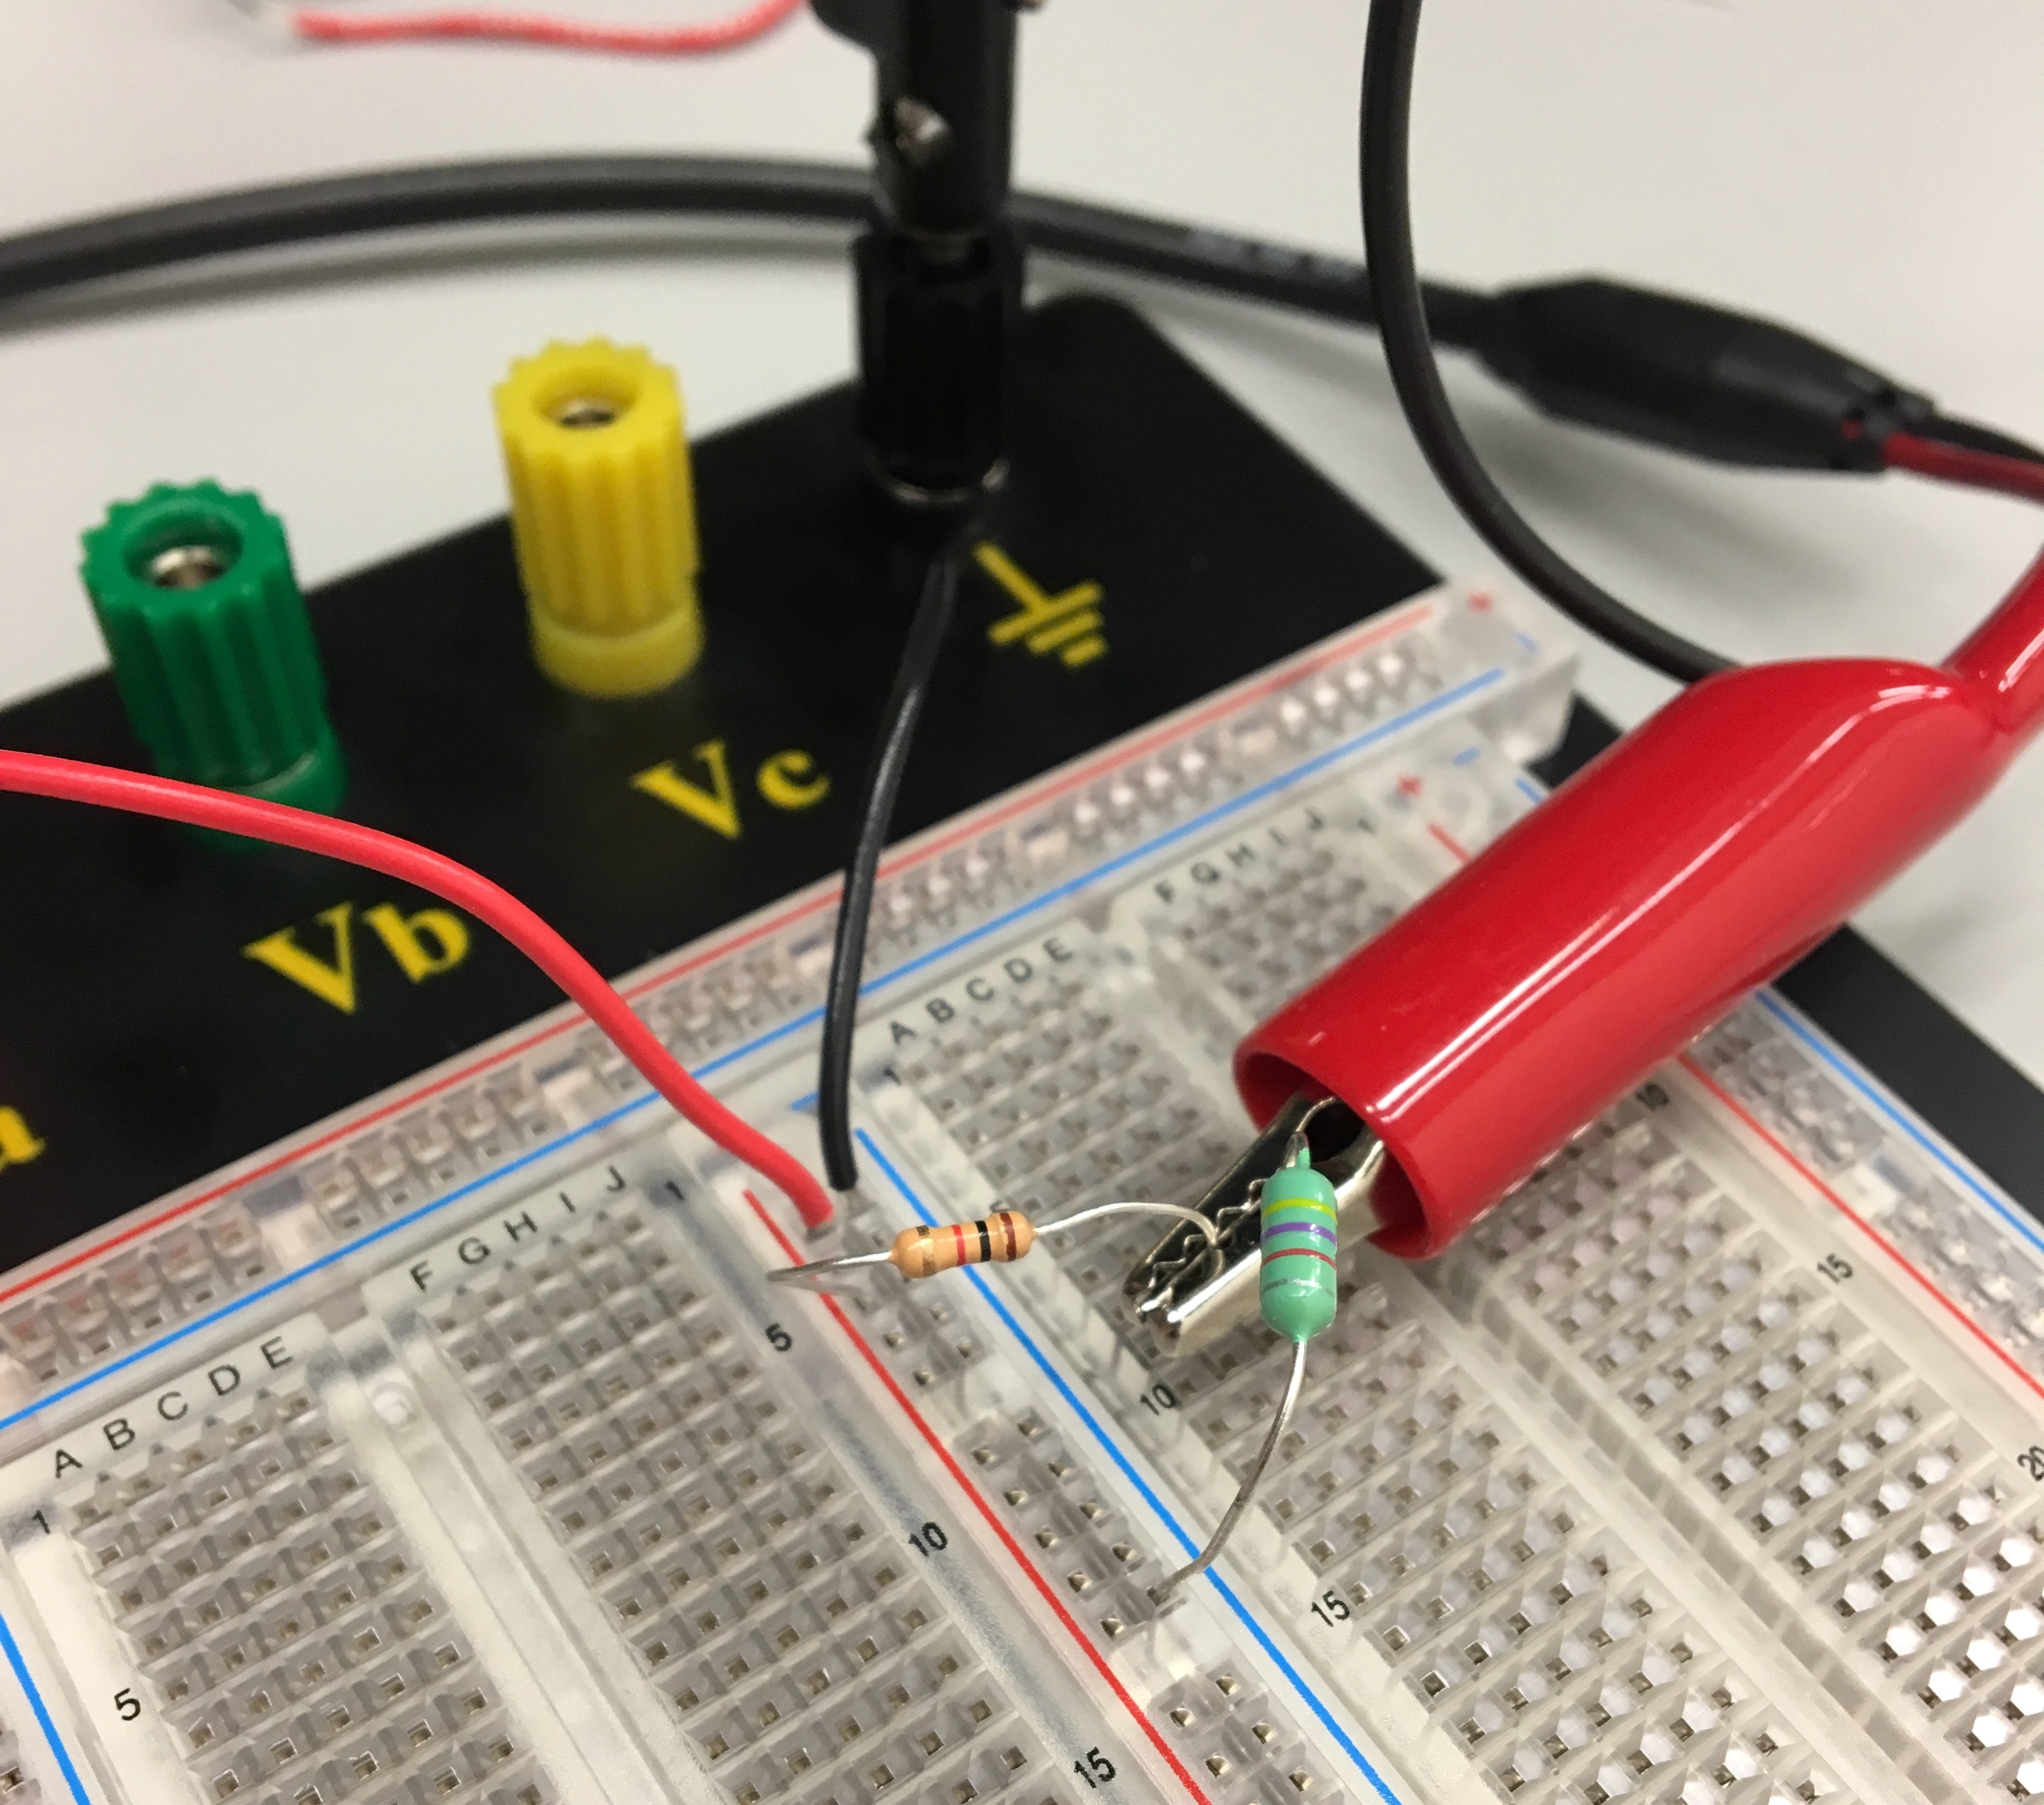
\includegraphics[width=\columnwidth]{images/lab8_circ2.jpg}
    \captionof{figure}{Circuit 2}
    \label{fig:circ2image}
    \medskip
\endgroup



%%%%%%%%%%%%%%%%%
%% RLC Circuit %%
%%%%%%%%%%%%%%%%%
\subsection{RLC Circuit}
\noindent In a RC circuit, inductor and capacitor {\color{red}does something something something theory theory Lorem ipsum dolor sit amet, consectetur adipiscing elit. Nullam ultrices feugiat risus eget tincidunt. Integer nibh erat, luctus sed consectetur eu, dapibus ac nisi.Lorem ipsum dolor s}

\begingroup
    \centering
    \medskip
    %width=\columnwidth
    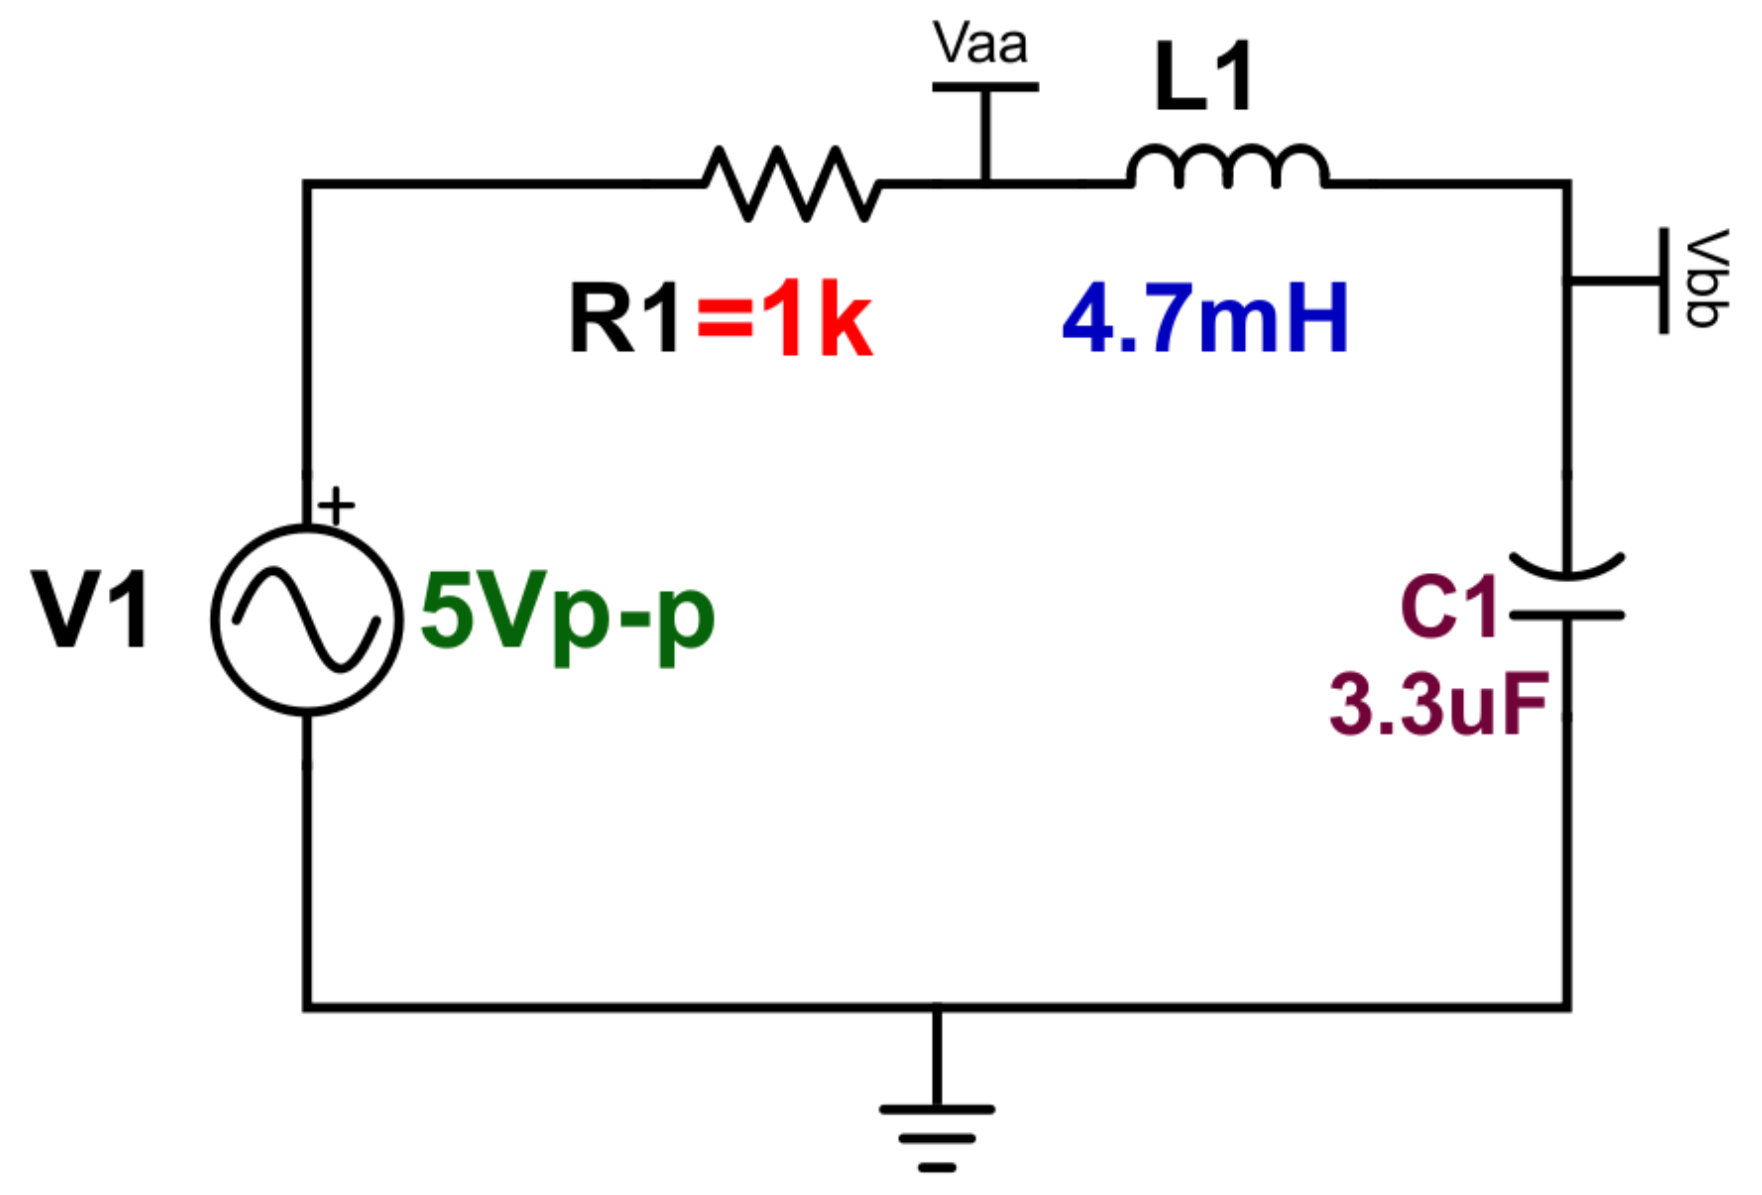
\includegraphics[width=\columnwidth]{images/lab8_circuit3.png}
    \captionof{figure}{Circuit 3}
    \label{fig:circ3}
    \medskip
\endgroup

\noindent Finally the last circuit was built on the breadboard by using the provided schematics (Figure \ref{fig:circ3}). One 1K resistor, one 4.7 $mH$ inductor, and one 3.3 $uF$ capacitor was used along the AC wave generator. This time oscilloscope was attached to both inductor's leg and capacitor's leg. Once the circuit was completed (Figure \ref{fig:circ3image}), 5V p-p and 1kHz AC voltage was applied to the circuit and generated waveforms in the circuit were captured. Later, the frequency of the applied voltage was increased until 40 kHz to observe the phase differences in the circuit.

\begingroup
    \centering
    \medskip
    %width=\columnwidth
    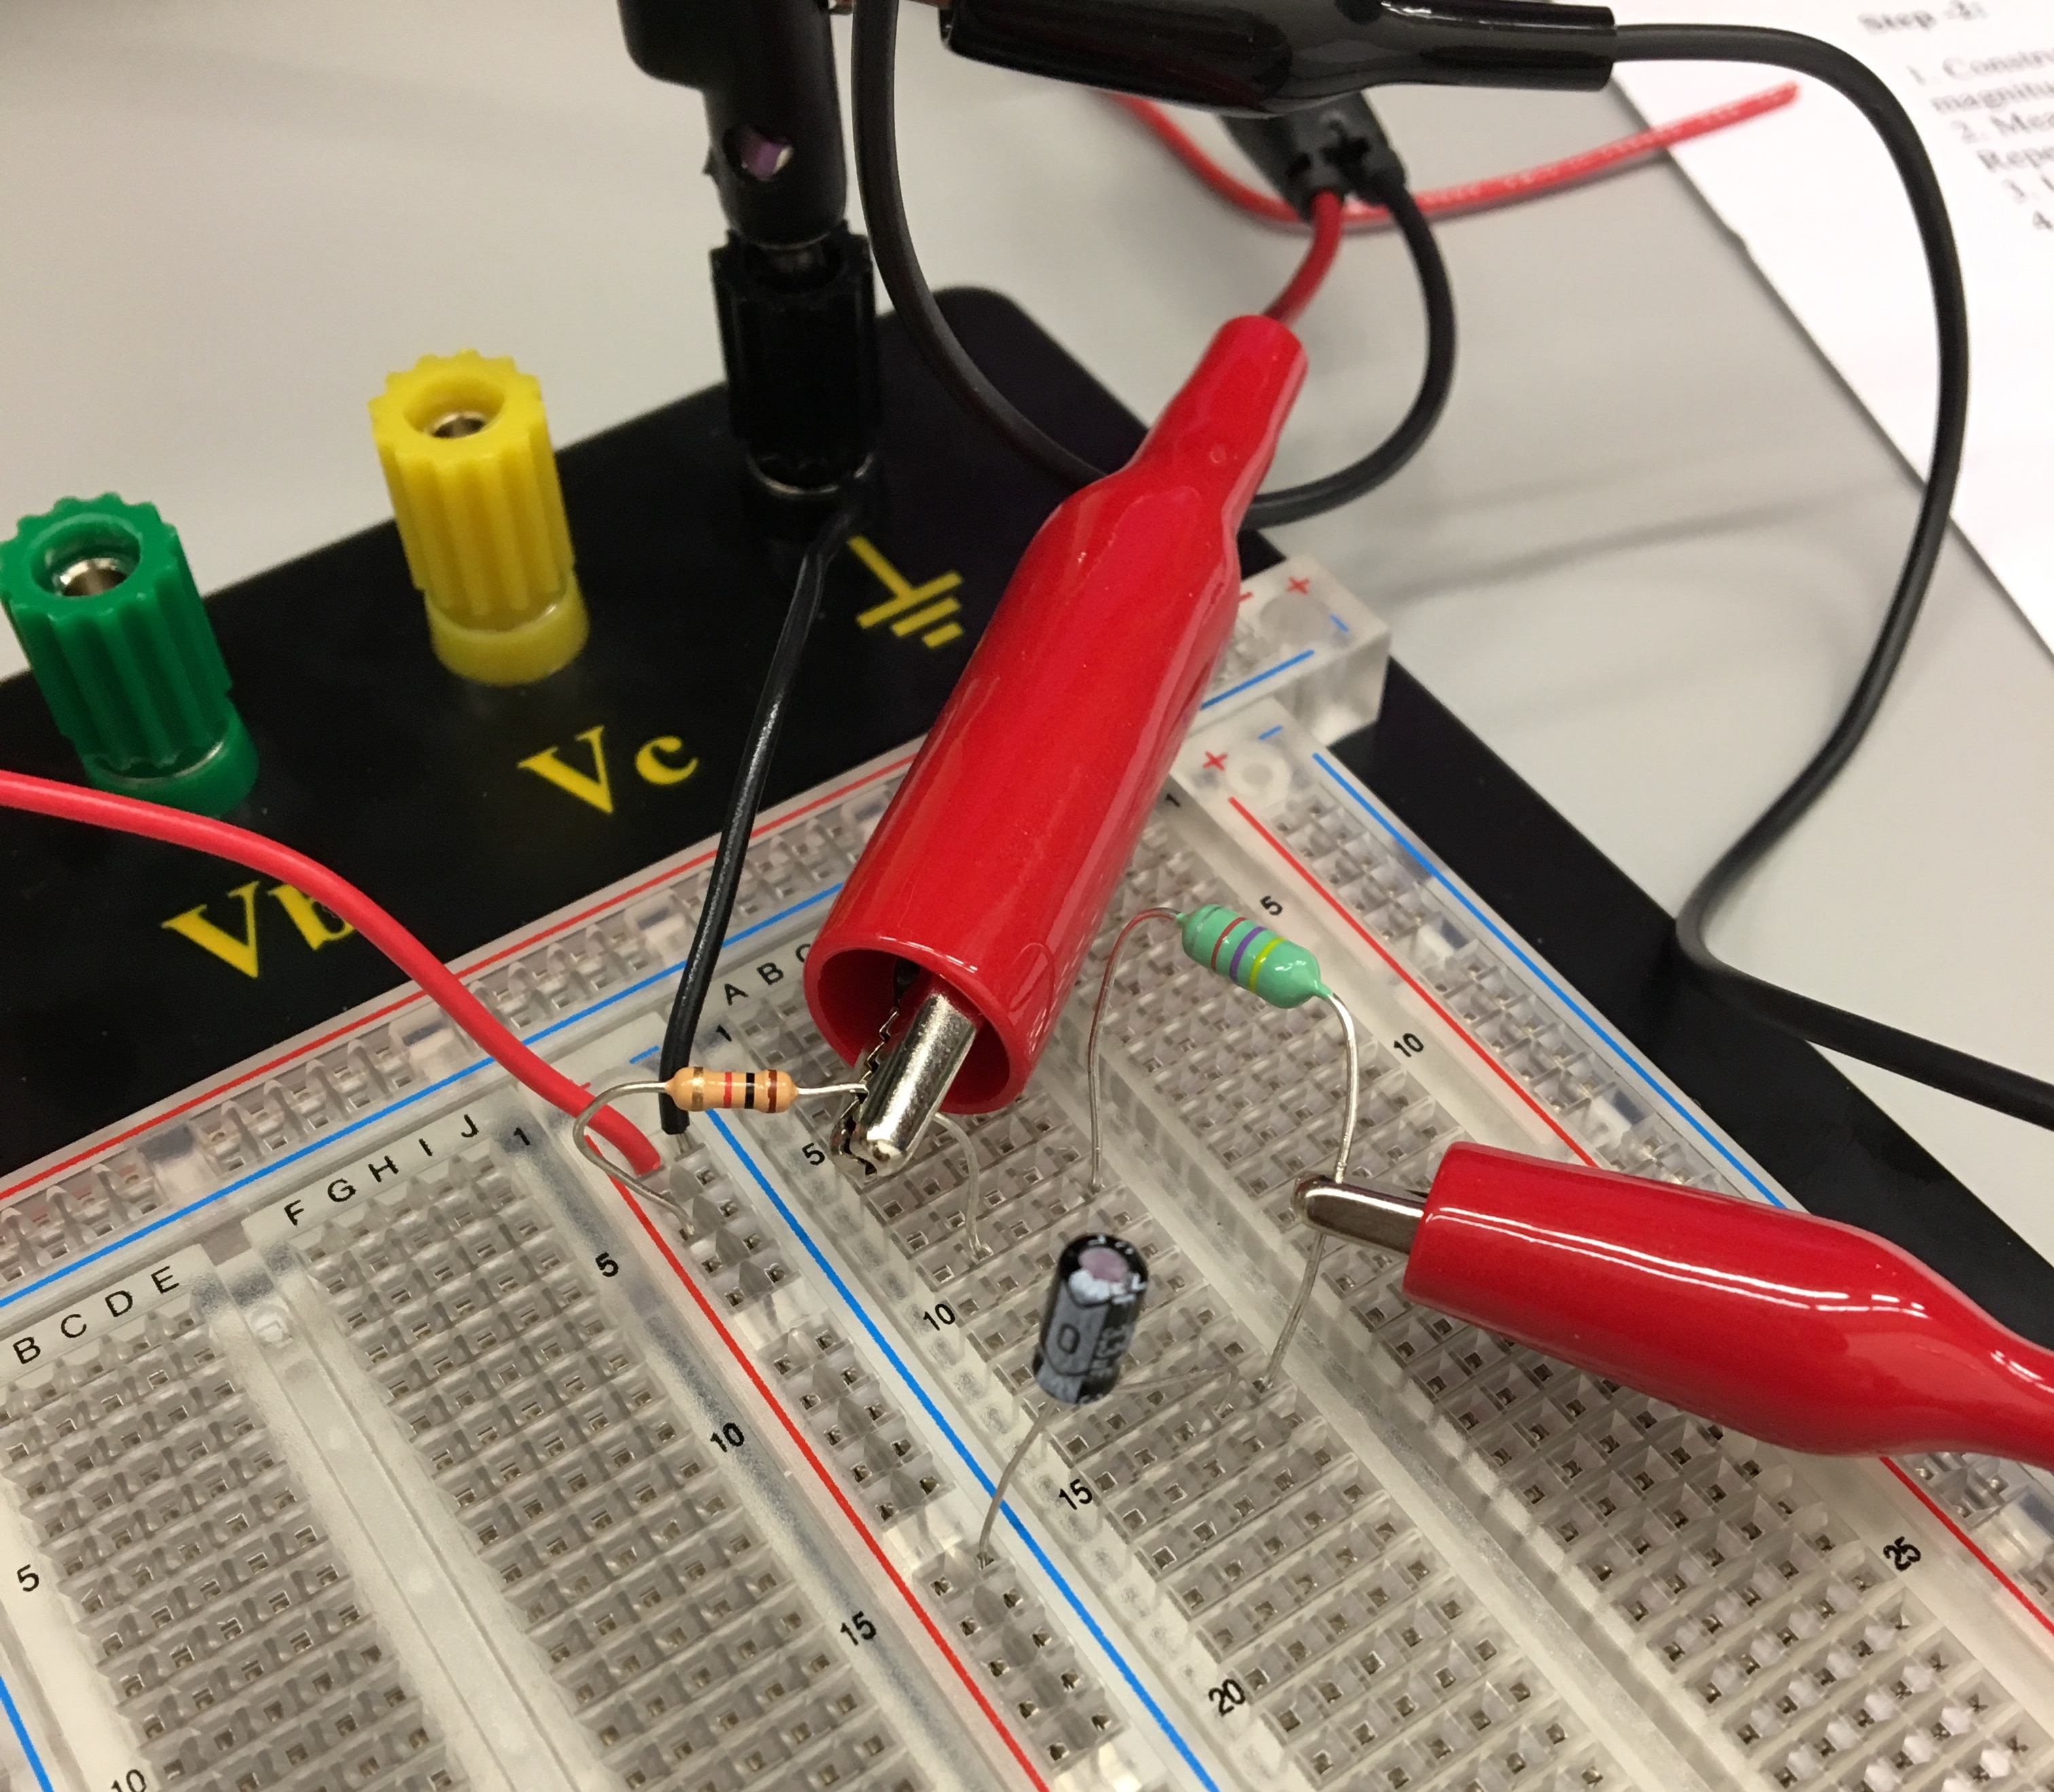
\includegraphics[width=\columnwidth]{images/lab8_circ3.jpg}
    \captionof{figure}{Circuit 3}
    \label{fig:circ3image}
    \medskip
\endgroup

\pagebreak

\section{Results and Discussion}

\noindent All configurations operated as expected and the results of each circuit configuration was recorded in the the tables and the observed wave forms were screenshot. Green lines represents the signal directly coming from the AC function generator and yellow\&purple lines represent the signal captured from legs of the capacitor\&inductor in the oscilloscope screenshots.

%%%%%%%%%%%%%%%%
%% RC Circuit %%
%%%%%%%%%%%%%%%%
\subsection{RC Circuit}
\noindent {\color{red} Some explanation ething theory theory Lorem ipsum dolor sit amet, consectetur adipiscing elit. Nullam ultrices feugiat risus eget tincidunt. Integer nibh erat, luctus sed consectetur eu, dapibus ac nisi.Lorem ipsum } \\

\begingroup
\bigskip
    \centering
    \def\arraystretch{1.5}
    \begin{tabular}{ccccc}
        \toprule
        Frequency (kHz) & Vin (V) & Vout (mV) & \thead{Phase \\ Difference (\degree)}\\
        \midrule
        1 & 5 & 254 & 74\\
        2 & 5 & 150 & 72\\
        \bottomrule
    \end{tabular}
    \captionof{figure}{Tabulation of the measurements for the RC circuit built with 1K\ohm \, resistor and 3.3$uF$ capacitor}
    \label{fig:rctable}
\medskip
\endgroup

\begingroup
    \centering
    \medskip
    %width=\columnwidth
    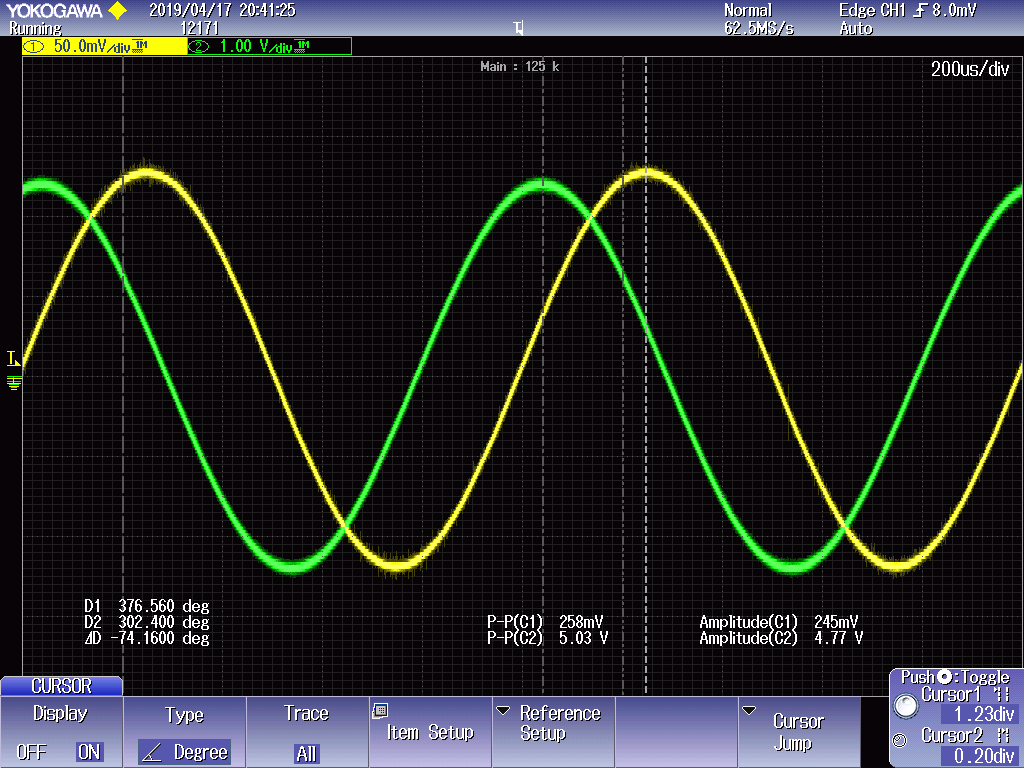
\includegraphics[width=\columnwidth]{images/lab8_002.png}
    \captionof{figure}{Phase shift of the RC circuit at 1 kHz}
    \label{fig:rcosc1}
    \medskip
\endgroup

\begingroup
    \centering
    \medskip
    %width=\columnwidth
    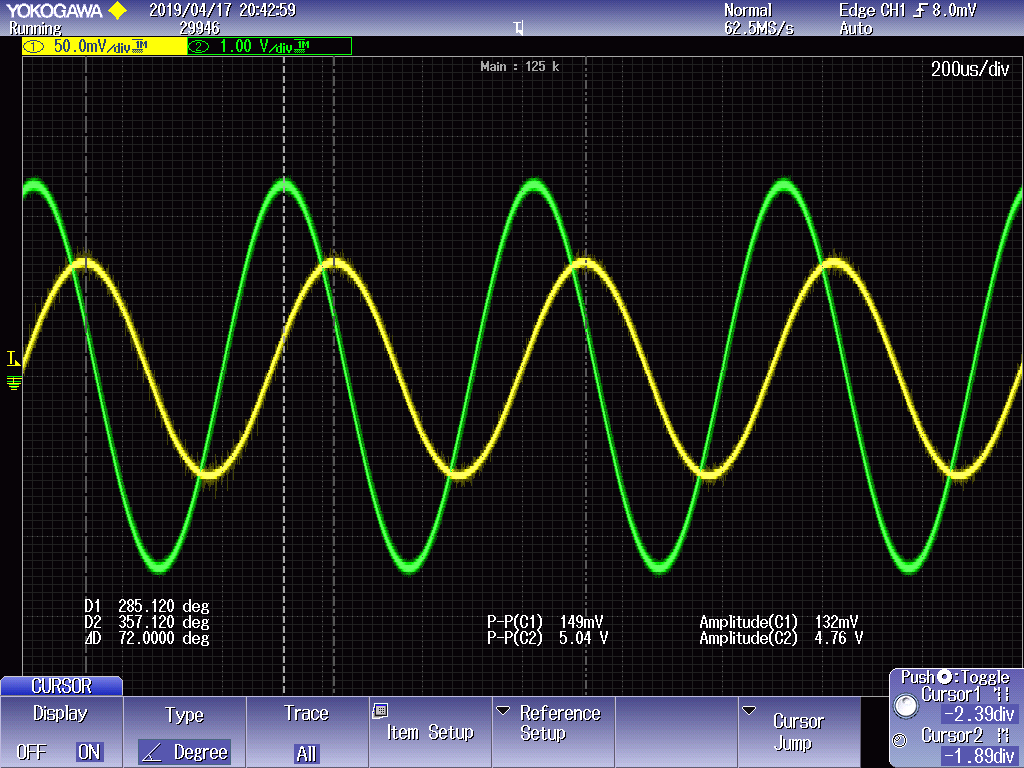
\includegraphics[width=\columnwidth]{images/lab8_005.png}
    \captionof{figure}{Phase shift of the RC circuit at 2 kHz}
    \label{fig:rcosc2}
    \medskip
\endgroup


%%%%%%%%%%%%%%%%
%% RL Circuit %%
%%%%%%%%%%%%%%%%
\subsection{RL Circuit}
\noindent {\color{red} Some explanation ething theory theory Lorem ipsum dolor sit amet, consectetur adipiscing elit. Nullam ultrices feugiat risus eget tincidunt. Integer nibh erat, luctus sed consectetur eu, dapibus ac nisi.Lorem ipsum } \\

\begingroup
\bigskip
    \centering
    \def\arraystretch{1.5}
    \begin{tabular}{ccccc}
        \toprule
        Frequency (kHz) & Vin (V) & Vout (mV) & \thead{Phase \\ Difference (\degree)}\\
        \midrule
        1 & 5 & 220 & -40\\
        2 & 5 & 320 & -50\\
        \bottomrule
    \end{tabular}
    \captionof{figure}{Tabulation of the measurements for the RC circuit built with 1K\ohm \, resistor and 4.7$mH$ inductor}
    \label{fig:rltable}
\medskip
\endgroup

\begingroup
    \centering
    \medskip
    %width=\columnwidth
    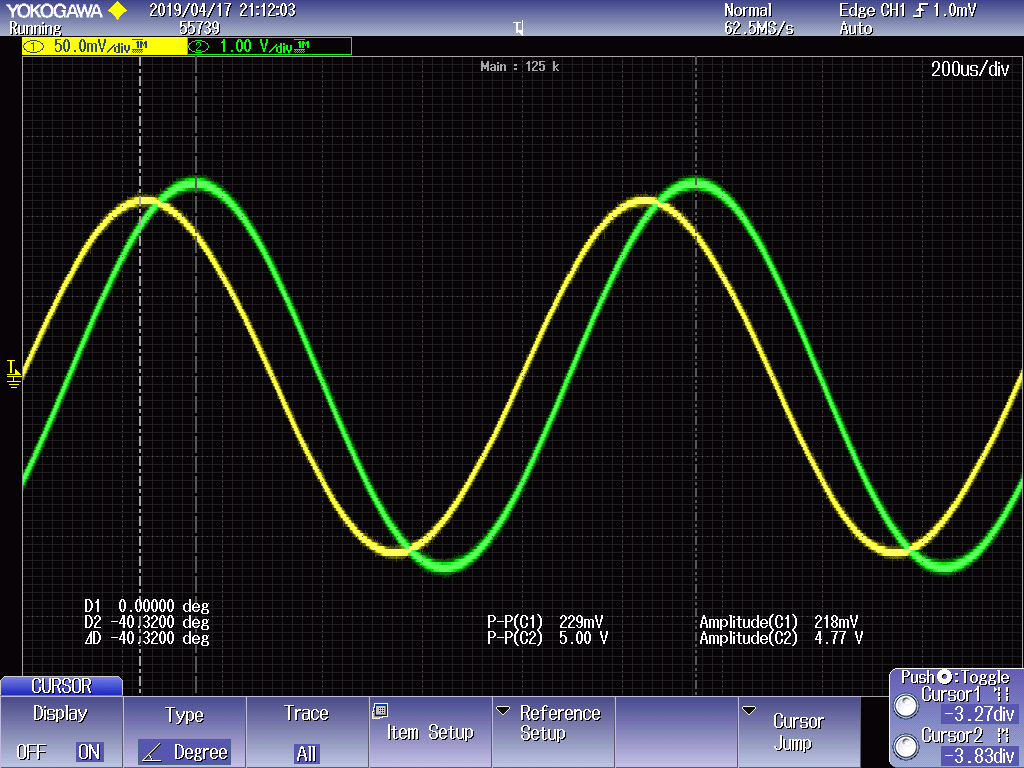
\includegraphics[width=\columnwidth]{images/lab8_014.png}
    \captionof{figure}{Phase shift of the RL circuit at 1 kHz}
    \label{fig:rlosc1}
    \medskip
\endgroup

\begingroup
    \centering
    \medskip
    %width=\columnwidth
    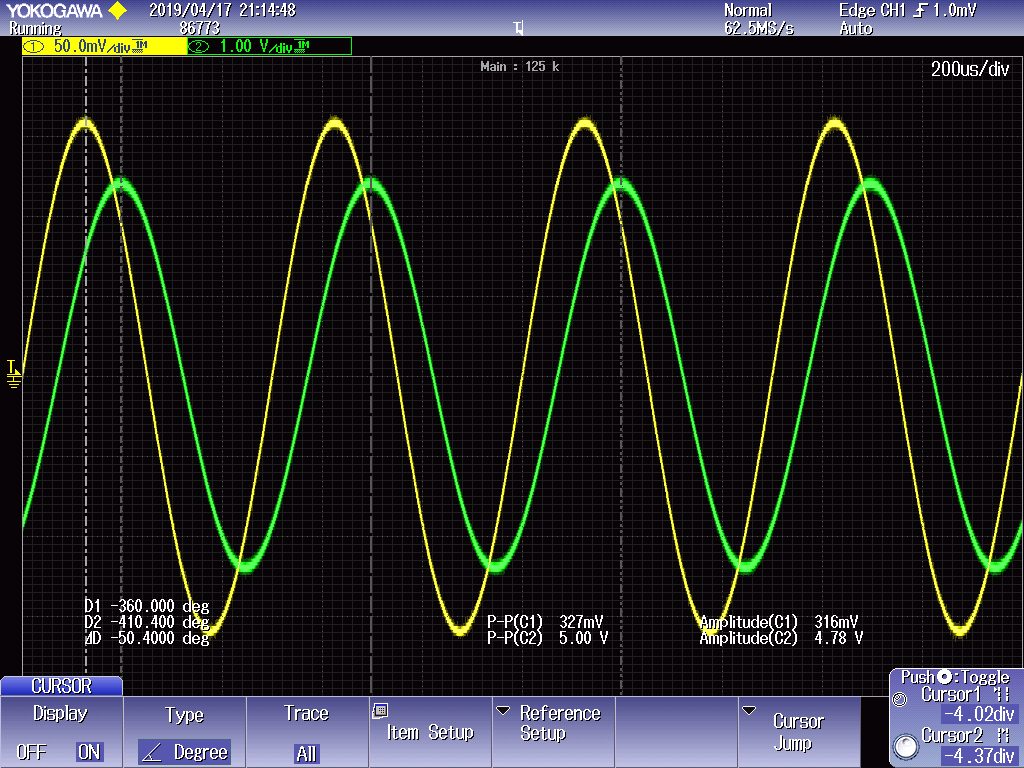
\includegraphics[width=\columnwidth]{images/lab8_017.png}
    \captionof{figure}{Phase shift of the RL circuit at 2 kHz}
    \label{fig:rlosc2}
    \medskip
\endgroup


%%%%%%%%%%%%%%%%%
%% RCL Circuit %%
%%%%%%%%%%%%%%%%%
\subsection{RCL Circuit}
\noindent {\color{red} Some explanation ething theory theory Lorem ipsum dolor sit amet, consectetur adipiscing elit. Nullam ultrices feugiat risus eget tincidunt. Integer nibh erat, luctus sed consectetur eu, dapibus ac nisi.Lorem ipsum } \\

\begingroup
\bigskip
    \centering
    \def\arraystretch{1.5}
    \begin{tabular}{cccccc}
        \toprule
        \thead{Output} & \thead{Frequency\\(kHz)} & \thead{Vin\\(V)} & \thead{Vout\\(mV)} &\thead{Phase \\ Difference (\degree)} \\
        \midrule
        Vaa & 1 & 5 & 260 & 20\\
        Vbb & 1 & 5 & 250 & 72\\
        \bottomrule
    \end{tabular}
    \captionof{figure}{Tabulation of the measurements for the RLC circuit built with 1K\ohm \, resistor, 4.7$mH$ inductor, and 3.3$uF$ capacitor}
    \label{fig:rcltable}
\medskip
\endgroup

\begingroup
    \centering
    \medskip
    %width=\columnwidth
    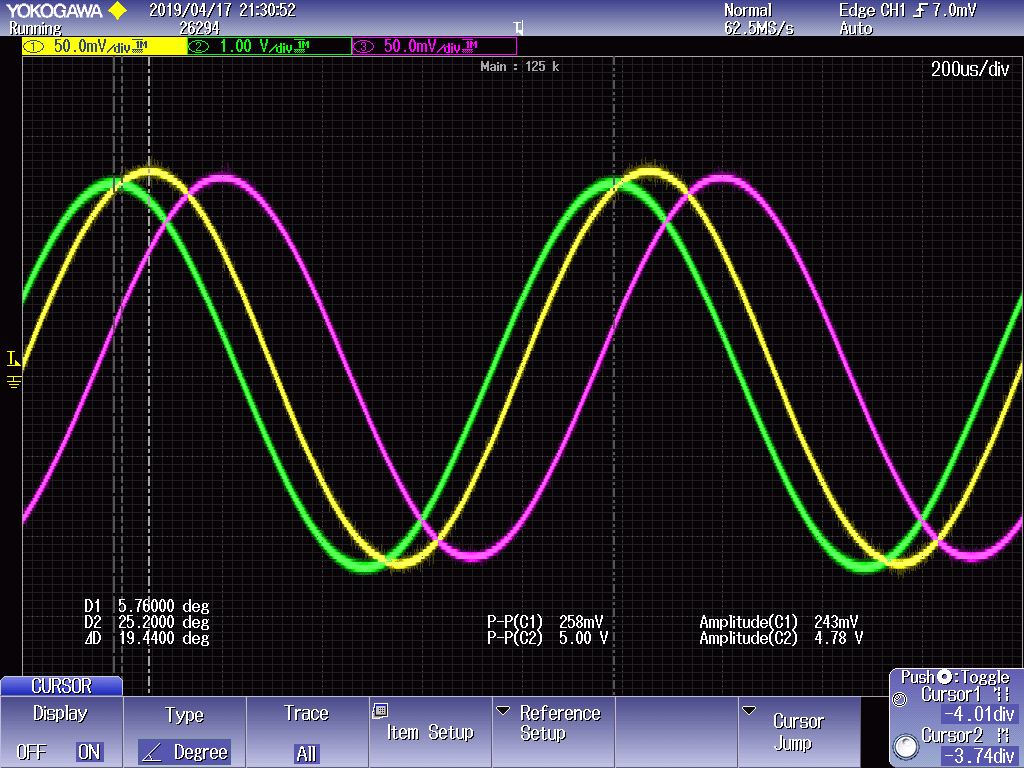
\includegraphics[width=\columnwidth]{images/lab8_025.png}
    \captionof{figure}{Phase shift of the RL circuit at 1 kHz. Yellow line represents the signal captured from inductor while purple line represents the signal captured from capacitor.}
    \label{fig:rclosc1}
    \medskip
\endgroup

%%%%%%%%%%%%%%%%%%%%%%%%%%
%% General Observations %%
%%%%%%%%%%%%%%%%%%%%%%%%%%
\subsection{General Observations}

\noindent {\color{red}some text related to the phasor calculations and their results psum dolor sit amet, consectetur adipiscing elit. Nullam ultrices feugiat risus eget tincidunt. Integer nibh erat, luctus sed consectetur eu, dapibus ac nisi.Lorem ipsum dolor sit amet, consectetur adipiscing elit. Nullam ultrices feugiat risus eget tincidunt. Integer nibh erat, luctus sed consectetur eu, dapibus ac nisi. Integer nibh erat, luctus sed consectetur eu, dapibus ac nisi.Integer nibh erat, luctus sed consectetur eu, dapibus ac nisi.} \\

\noindent Figures \ref{fig:phaseshift1} and \ref{fig:phaseshift40} demonstrate how phase shift changes as the frequency of the voltage source increases. \\

\begingroup
    \centering
    \medskip
    %width=\columnwidth
    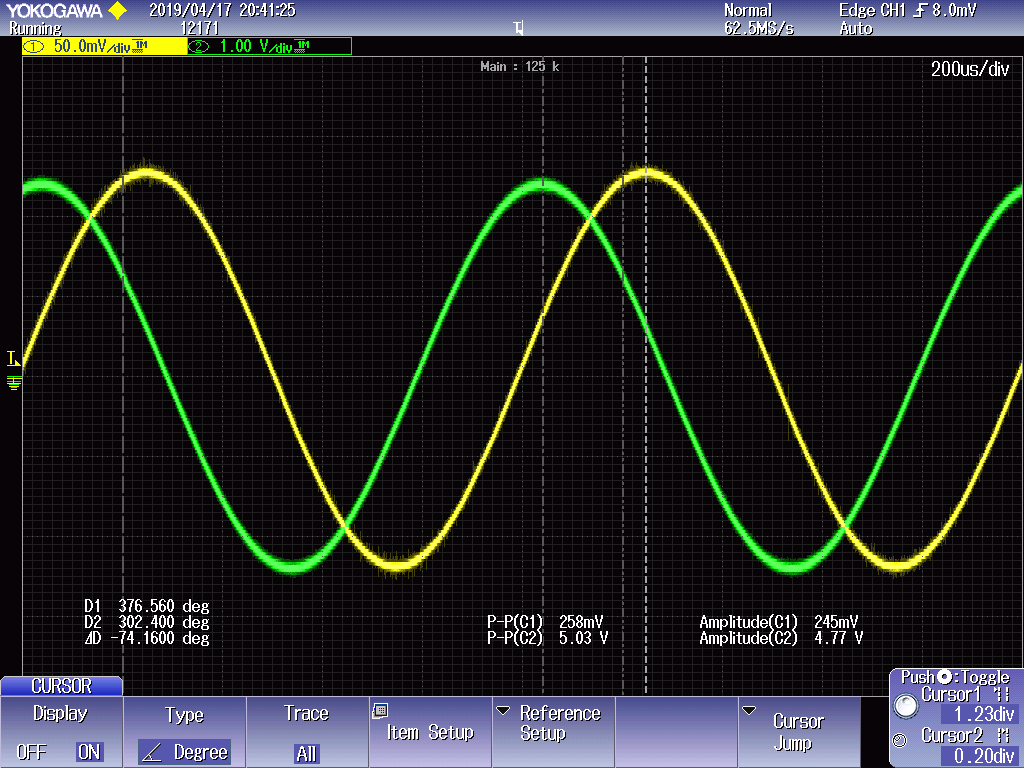
\includegraphics[width=\columnwidth]{images/lab8_002.png}
    \captionof{figure}{Phase shift at 1 kHz}
    \label{fig:phaseshift1}
    \medskip
\endgroup

\begingroup
    \centering
    \medskip
    %width=\columnwidth
    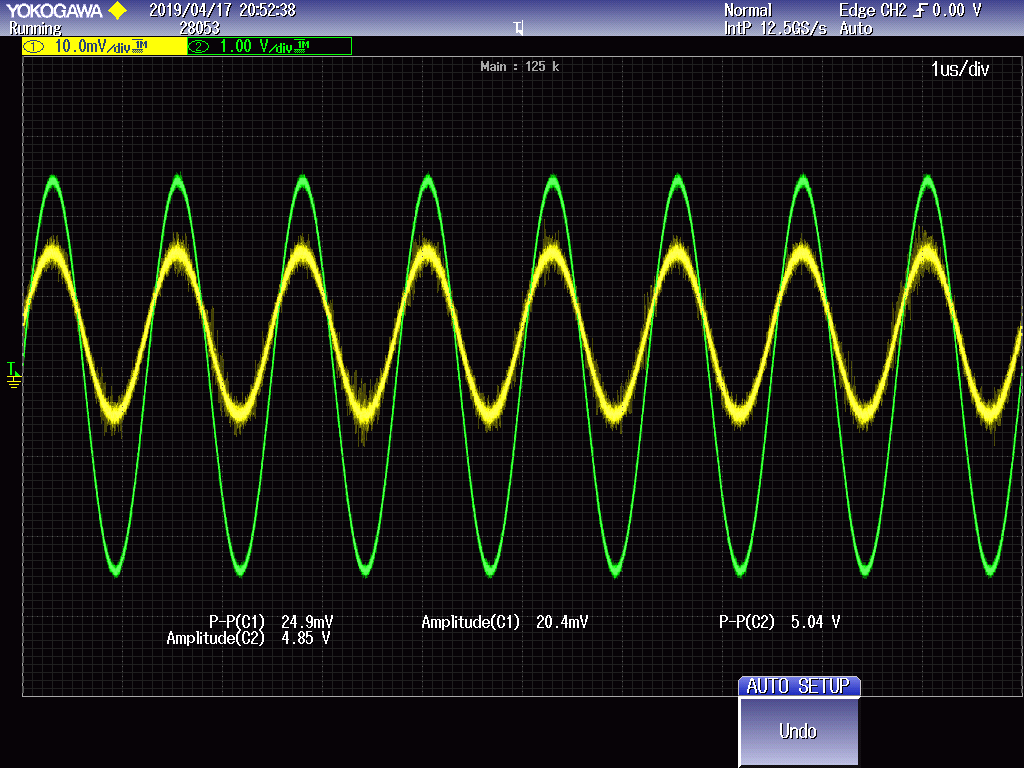
\includegraphics[width=\columnwidth]{images/lab8_012.png}
    \captionof{figure}{Phase shift at 40 kHz}
    \label{fig:phaseshift40}
    \medskip
\endgroup

\section{Conclusions}
% Understanding and applications
\noindent We learned two


\printbibliography

\end{document}